\subsection{Results}
\label{subsec:results}

% BEGIN GENERATED tab:main_results (full_run_28092026/paper_results.py --write)
\begin{table*}[t]
\centering
\small
\begin{tabular}{l r c c r c c}
\toprule
\rowcolor{gray!10}
\textbf{Model} & \textbf{FAC} & \textbf{95\% CI} & \textbf{Tier} & \textbf{MC} & \textbf{95\% CI} & \textbf{Tier} \\
\midrule
\texttt{DeepSeek V4.1 Flash} & 0.976 & 0.957--0.990 & ab & 0.897 & 0.870--0.922 & ab \\
\texttt{Kimi K3} & 0.974 & 0.956--0.988 & ab & 0.915 & 0.893--0.936 & ac \\
\texttt{Claude Sonnet 5} & 0.972 & 0.952--0.988 & ab & 0.922 & 0.902--0.942 & c \\
\texttt{GLM-5.3-Flash} & 0.969 & 0.947--0.986 & a & 0.912 & 0.885--0.936 & ac \\
\texttt{Muse Glimmer 30B} & 0.967 & 0.946--0.984 & ab & 0.898 & 0.872--0.923 & abc \\
\texttt{GLM-5.3}$^{\dagger}$ & 0.948 & 0.918--0.973 & b & 0.901 & 0.866--0.931 & abcd \\
\texttt{Qwen3-235B-2507}$^{\ast}$ & 0.886 & 0.852--0.916 & c & 0.893 & 0.868--0.916 & ab \\
\texttt{Gemini 3.1 Flash-Lite}$^{\ast}$ & 0.872 & 0.829--0.911 & cd & 0.864 & 0.834--0.893 & de \\
\texttt{Gemma 4 26B}$^{\ast}$ & 0.864 & 0.825--0.899 & cd & 0.876 & 0.848--0.903 & bd \\
\texttt{GPT-5.4 mini}$^{\ast}$ & 0.847 & 0.806--0.885 & cd & 0.833 & 0.796--0.869 & ef \\
\texttt{gpt-oss-20b} & 0.814 & 0.770--0.856 & d & 0.816 & 0.778--0.851 & f \\
\bottomrule
\end{tabular}
\caption{\textbf{Final Answer Accuracy and Milestone Coverage.} FAC over the 2,250 instances and MC over the 147 templates with milestones, each with a 95\% interval that resamples templates, in order of FAC. Models that share a letter in a tier column do not differ on that measure after Holm correction over the 55 pairs; the letters are a compact letter display~\citep{piepho2004letter}. $^{\ast}$Returns no reasoning tokens at its provider's defaults. $^{\dagger}$100 responses are empty at the output ceiling and score 0.}
\label{tab:main_results}
\end{table*}
% END GENERATED tab:main_results

\paragraph{Final Answer Accuracy.}
The final answer separates the tiers of models but not the models within the top tier.
\autoref{tab:main_results} gives each model's Final Answer Accuracy (FAC) and Milestone Coverage
(MC) with 95\% intervals and a compact letter display~\citep{piepho2004letter}: models that share a
letter do not differ after Holm correction over the 55 pairs.
FAC runs from 0.814 (\texttt{gpt-oss-20b}) to 0.976 (\texttt{DeepSeek V4.1 Flash}).
Five models lie within 0.009 of one another, between 0.967 and 0.976, and no pair among them
differs: they form one tier with no order inside it and are not separable at this size.
\texttt{GLM-5.3} (0.948) follows and differs from only one of the five (\texttt{GLM-5.3-Flash}); 100
of its responses are empty at the output ceiling and score 0.
The remaining five models lie between 0.814 and 0.886, and each differs from every model of the top
six.
In all, 32 of the 55 pairs differ after correction, and the 23 that do not all lie below the
smallest difference the design detects at 80\% power (0.010 to 0.065, depending on the pair).
Four of the five lowest scores belong to the four models that return no reasoning tokens at their
providers' defaults; with reasoning at medium effort on the 450-instance subset,
\texttt{GPT-5.4 mini} moves from 0.858 to 0.951 (95\% CI of the change 0.056 to 0.133) and
\texttt{Gemini 3.1 Flash-Lite} from 0.874 to 0.890 ($-0.010$ to 0.042), less than the design
detects.
Instances of a template mostly share one fate: 57 to 130 of the 150 templates per model have the
same score on all 15 instances.
\autoref{appendix:results} gives the extended table, every pairwise comparison for both measures,
and the per-template variance.

\paragraph{Difficulty.}
Every model scores lower on Advanced than on Easy templates, by 0.055 to 0.199, but the gap is
significant after correction for four of the eleven models, and for none once two Advanced chemical
templates whose wording does not pin the answer are set aside.
The four are the lowest-scoring models, \texttt{Gemini 3.1 Flash-Lite}, \texttt{Gemma 4 26B},
\texttt{GPT-5.4 mini}, and \texttt{gpt-oss-20b} (gaps 0.151 to 0.199), three of which run without
reasoning tokens; the top five models' gaps are 0.055 to 0.073, with intervals that all exclude zero
but do not survive correction, against detectable gaps of 0.080 to 0.177.
\texttt{GLM-5.3}'s gap of 0.134 is mostly an output-ceiling effect: its empty responses fall on
Advanced templates, and without them the gap is 0.010.
Three chemical domain experts read the two templates: one asks for the work of compressing a gas
without saying whether the system is closed or flowing, two readings whose answers differ by more
than the tolerance, and the other's answer depends on the thermochemical data source by more than
the tolerance.
Without these two templates the gaps are 0.029 to 0.157 and none holds after correction.
Across branches, one pair in the whole evaluation separates after correction (\texttt{gpt-oss-20b},
electrical above civil), so we report branch and domain means without ranking them
(\autoref{appendix:results}).

\paragraph{Milestone Coverage.}
MC runs from 0.816 to 0.922 and orders the models differently from FAC (Kendall's $\tau$ 0.709, 95\%
CI 0.514 to 0.855~\citep{kendall1938}).
\texttt{Claude Sonnet 5} is first on MC and third on FAC; \texttt{DeepSeek V4.1 Flash} is first on
FAC and sixth on MC, 0.025 below \texttt{Claude Sonnet 5} (Holm-adjusted $p = 0.024$), a pair that
FAC does not separate.
Over the 55 pairs, 28 differ after correction under the sign-flip test and 29 under a Wilcoxon
signed-rank test~\citep{wilcoxon1945}, the two agreeing on 52 pairs; the three models highest on MC,
\texttt{Claude Sonnet 5}, \texttt{Kimi K3}, and \texttt{GLM-5.3-Flash}, do not separate from one
another.
MC credits stated intermediates: it does not rise with the number of steps a model writes
(Spearman's $\rho$~\citep{spearman1904} between a template's mean coverage and its mean number of
steps is $-0.11$ to $-0.26$ for every model), and it ranks what responses state, not how soundly
they reason, so we read no trade-off into the two orderings.

\paragraph{Coverage on Wrong Answers.}
Most wrong answers are late failures of a derivation that is largely there, not absent derivations.
On readable wrong answers, matching alone finds 44\% to 81\% of the milestones, against a chance
floor of 10\% to 22\% (the same response matched against a sibling instance's milestones); with the
judge the share is 46\% to 85\%, the 85\% resting on the 7 wrong answers of \texttt{GLM-5.3}.
Among the five models with more than 100 wrong answers, 13\% to 26\% of them reach every milestone:
a complete derivation to a wrong value.
On answered wrong answers, a milestone the judge rules missing points at the failure in 14\% to 79\%
of responses, a judged step flag in 14\% to 89\%, and an arithmetic flag in 0\% to 48\%, depending
on the model; these are shares of responses with a flag, not diagnoses (\autoref{appendix:results}).

\paragraph{Step-Level Diagnostics.}
Some correct answers contain flawed steps, at rates the diagnostics flag but do not count.
The arithmetic check flags 0.5\% to 22.5\% of correct-answer responses, at a precision of 0.905 on
these models (171 of 189 flags that a domain expert read were slips), and the judged step check
flags 1.1\% to 22.0\%, at a precision of 0.70 and a recall of 0.36 inside correct-answer responses
in the expert study.
These rates do not rank the models: the arithmetic check reads 2.8 to 9.8 displayed calculations per
response, depending on how much arithmetic a model writes out, so \texttt{Qwen3-235B-2507}'s 22.5\%
comes with 9.8 calculations per response and \texttt{DeepSeek V4.1 Flash}'s 0.5\% with 3.3; and with
recall below one half, a flag rate is neither a count of slips nor a share of correct answers that
rest on flawed reasoning (\autoref{appendix:results}).

\paragraph{Consistency and Depth.}
Failure grows with the depth of the gold derivation: every model gets more answers wrong on
instances with six or more milestones than on one-milestone instances, with wrong-answer rates of
0.037 to 0.291 against 0.000 to 0.045 (the milestone count is the template's, not a difficulty
label).
Within a template, the six strongest models solve all 15 instances of 84\% to 91\% of the 58
single-path templates, whereas four of the five weakest solve all instances of 36\% to 48\% of them
(\texttt{Gemini 3.1 Flash-Lite} 67\%) and some but not all instances of 48\% to 57\%; on a
single-path template every instance follows the same method, so a partly solved template is a
failure on the numbers, not the method (\autoref{appendix:results}).

\paragraph{Rewording.}
Fixed template wording does not inflate the scores by more than five points for ten of the eleven
models.
To test memorized wording, we rewrote one instance in five of every template (450 instances) with an
LLM from a family outside both the evaluated models and the judge, under rules that keep every
number, unit, symbol, formula, and part in place; 316 rewrites passed scripted checks, and a domain
expert of the instance's branch confirmed 277 of them, on 115 templates, as the same problem with
the same answer.
On these 277 pairs, the paired change in FAC lies between $-0.031$ and $+0.020$ across the eleven
models, and none is significant after correction; for ten models the 90\% interval lies within
$\pm 0.05$, a margin equal to the paired difference the design was planned to detect and fixed after
the point estimates were known, and for \texttt{Qwen3-235B-2507} it reaches $-0.067$, so a
five-point drop is not ruled out for that model.
MC changes by the same small amounts.
The models' ordering on the paraphrases agrees with their ordering on the originals with
$\tau = 0.673$ (0.455 to 0.881), at the lower edge of what sampling alone produces at this size
(median 0.782): the tiers hold under rewording, and the order within the top tier is not resolved.
The expert step was necessary: the experts rejected 39 of the 316 pairs that passed every scripted
check (12\%), almost always for a dropped or altered qualifier that changes the physics or the asked
quantity.
The test bounds memorized wording, not memorized methods, since numbers and problem structure are
kept, and it covers the 115 templates whose problems could be reworded without loss.
For comparison, on 300 instances decoded three times, four models' FAC has a standard deviation of
0.004 to 0.013 across repeats, and 86\% to 94\% of instances receive the same verdict every time.
The ordering is also unchanged at half and double the answer tolerance ($\tau = 0.927$), and FAC
moves by at most 0.004 without the four templates whose answers can be read off the question's
wording and by $-0.004$ to $+0.008$ without the nine symbolic-answer templates
(\autoref{appendix:rewording} and~\autoref{appendix:results}).

\paragraph{Flagship Anchors, Governing Equations, and a Code Tool.}
On the 450-instance subset, two flagships that pass the selection rule do not exceed the top tier,
and neither the governing equations nor a code tool moves the two closed models tested beyond five
points.
\texttt{DeepSeek V4 Pro} scores 0.968 (0.950 to 0.983), and \texttt{GPT-5.4} scores 0.980 (0.964 to
0.993) with reasoning at medium effort and 0.941 (0.909 to 0.969) at its provider's default, which
returns no reasoning tokens; the top five on the same instances score 0.964 to 0.976, with intervals
that contain both reasoning anchors, and on Advanced templates 0.92 to 0.95 against the anchors'
0.87 to 0.95.
Supplying each template's governing equations with the question (405 instances of the 135 templates
that state them in symbols) lifts \texttt{gpt-oss-20b} by 0.064 (0.027 to 0.104), partly because
fewer responses run out of room (0.043 on the instances answered in both conditions), and changes
\texttt{GPT-5.4 mini} ($-0.019$) and \texttt{Claude Sonnet 5} ($+0.007$) by amounts bounded within
$\pm 0.05$, while MC rises by 0.03 to 0.06 for all three.
Offered a Python tool with the prompt otherwise unchanged, \texttt{Claude Sonnet 5} calls it on 66\%
of instances and \texttt{GPT-5.4 mini} on 19\%, and neither model's FAC ($+0.004$; $-0.004$) or MC
changes beyond $\pm 0.05$; \texttt{GPT-5.4 mini}'s arithmetic flags on correct answers fall from
0.127 to 0.093.
The equations condition supplies no data tables, and the tool condition covers the two closed models
only, because no endpoint our provider rule admits served the open-weights model's tool calls
(\autoref{appendix:conditions}).

\subsection{Error Analysis}
\label{subsec:error_analysis}

\begin{figure}[t]
    \centering
    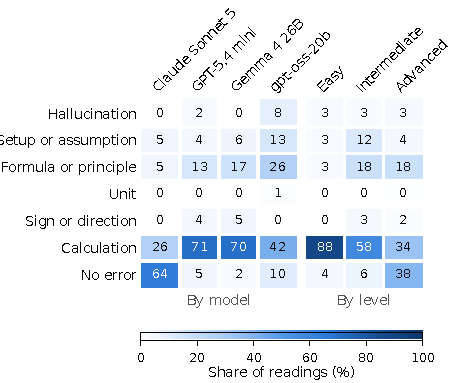
\includegraphics[width=\columnwidth]{figs/error-categories.pdf}
    \caption{\textbf{Error Categories of the Wrong Answers Read.} Three domain experts' 480 readings
    of 160 wrong answers, as the share of each column's readings in each category, by model (40
    wrong answers each) and by level (78, 186, and 216 readings); the categories run from the most
    to the least fundamental, and darker cells hold larger shares.}
    \label{fig:error_categories}
\end{figure}

\paragraph{Expert Reading of Wrong Answers.}
At the top of the ranking most remaining wrong answers are not reasoning errors; below it they are
mostly calculation slips, and wrong formulas or principles grow with difficulty.
Three domain experts read each of 160 wrong answers, 40 from each of four models that contrast the
tiers (\texttt{Claude Sonnet 5}, \texttt{GPT-5.4 mini}, \texttt{Gemma 4 26B}, and
\texttt{gpt-oss-20b}), drawn across levels in proportion to each model's wrong answers, and assigned
the first category that applies in a six-category hierarchy (hallucination, setup or assumption,
formula or principle, unit, sign, calculation) or ``no error'' (Fleiss'~$\kappa$
0.930~\citep{fleiss1971}); \autoref{fig:error_categories} shows the 480 readings by model and by
level.
For \texttt{Claude Sonnet 5}, 26 of 40 wrong answers are ``no error'' by majority: the answer is
correct or the question admits it, and the check cannot credit it.
For the other three models, calculation errors lead (28, 28, and 17 of 40), followed by formula or
principle errors (5, 7, and 9).
By level, the wrong answers on Easy problems are almost all calculation slips (69 of 78 readings),
whereas wrong formulas or principles are 18\% of the readings on Intermediate and Advanced problems
against 3\% on Easy ones.

\paragraph{What the Benchmark Discriminates.}
On final answers, the top five models solve the evaluation set almost completely (FAC 0.967 to
0.976; 0.92 to 0.93 on Advanced templates), and 122 of their 171 remaining incorrect verdicts are a
matter of form or of the question rather than of reasoning: symbolic answers, which we score by the
numbers they state, digits the question prescribes, and the two chemical templates.
The headroom therefore lies in the Advanced tier, in depth, in prescribed precision, and in the
process measures.
The limit of verification stands regardless: a response that computes correctly, misstates the rule
it applies, and lands the right answer passes every deterministic check
(\autoref{appendix:validation}), so the process measures earn their place on the wrong answers and
on the arithmetic behind the right ones.
\autoref{appendix:error_analysis} gives the taxonomy, the sample, the readers' agreement, the
per-model tables, and the templates whose wording does not pin the answer.
